
\chapter{The Quantized DEVS-LIM (QDL) Method}\label{chap:qdl}

The formal QDEVS function definitions for the proposed QDL method are presented in this chapter.

\section{QDL QDEVS Specification}

The original DEVS specification is outlined in \cite{zeigler2002}, and further developed for quantized systems (QDEVS) in \cite{zeigler1999}. The specification consists of several functions that need to be defined for a specific QDEVS model. These are

\begin{align*}
    f            & \text{:   Derivative Update function} \\
    \delta_{int} & \text{:   Internal State Transition Function} \\
    \delta_{ext} & \text{:   External State Transition Function} \\
    ta           & \text{:   Time Advance Function, and} \\
    Q            & \text{:   Quantization Function.}  \\
\end{align*}

These are defined below for the LIM atomic models presented in chapter \ref{chap:lim}, and for the LIQSS1 integration method in \cite{migoni2013}.

\subsection{QDL Derivative Update Function}

The derivative estimate is then determined from the LIM model for the nodes with

\begin{equation}\label{eq:d_func_node}
    d_i = \frac{H_{ii}}{C_{ii}} - \frac{G_{ii}}{C_{ii}} \cdot q_i + \frac{1}{C_{ii}} B_i \cdot q^{node} + \frac{1}{C_{ii}} \left(S_i - A_i\right) \cdot q^{branch},
\end{equation}

\noindent and for the branches with

\begin{equation}\label{eq:d_func_branch}
    d_k = \frac{E_{kk}}{L_{kk}} - \frac{R_{kk}}{L_{kk}} \cdot q_k + \frac{1}{L_{kk}} Z_k \cdot q^{node} + \frac{1}{L_{kk}} \left(T_k - A_k^T\right) \cdot q^{branch}, 
\end{equation}

\noindent where $C_{ii}$, $G_{ii}$, $H_{ii}$, $R_{kk}$, $L_{kk}$, and $E_{kk}$, are quantities from the LIM model at node $i$ and branch $k$. $B_i$, $S_i$, and $B_i$ are quantities from the LIM model at row $i$. $Z_k$, $T_k$, and $Z_k$ quantities from the LIM model at row $k$. $q_i$ is the quantized state at node $i$, $q_k$ is the quantized state at branch $k$, $q^{node}$ is the vector of node quantized states, and $q^{branch}$ is the vector of branch quantized states.

\subsection{QDL Internal State Transition Function} 

The internal state for each QDL atom is calculated by the internal transition function $\delta_{int}$. An internal transition occurs when the simulation time has advanced to the atom's $t^{next}$ value determined by its time advance function $ta$.

\noindent In this function, the node voltage states are updated as

\begin{equation}\label{eq:delta_int_node}
    v_i = v_i^{last} + d_i^{last} \cdot \left(t - t_i^{last}\right),
\end{equation}

\noindent and the branch currents are updated as

\begin{equation}\label{eq:delta_int_branch}
    i_k = i_k^{last} + d_k^{last} \cdot \left(t - t_k^{last}\right),
\end{equation}

\noindent where $v_i$ and $i_k$ are the voltage at node $i$ and the current at branch $k$ respectively.

\noindent After the states are updated, the $t^{last}$ values are saved:

\begin{equation} \label{eq:delta_int_save}
    t_i^{last} = t, \ \ t_k^{last} = t.
\end{equation}

\subsection{QDL External State Transition Function} 

In the case of QDL, the \emph{behavior} of the internal $\delta_{int}$ and the external $\delta_{ext}$ transition functions are identical. The difference is in how each is invoked. The internal transition is triggered when the simulation time $t$ has advanced to the atom's $t^{next}$ value determined in the $ta$ function, and the external transition is triggered when one or more connected atoms' quantized states change. Because the behavior of the internal and external transition functions is identical, the confluent transition function $\delta_{con}$ is not required.

\subsection{QDL Time Advance Function} 

The time until the next internal transition is determined from the time advance function $ta$. 

\noindent The time advance calculation for node $i$ is

\begin{equation} \label{eq:ta_node}
    t_i^{next} = 
    \begin{cases}
        t_i + ( \bar{q}_i - v_i ) \slash {d_i}, & \text{ if } d_i^{last} > 0 \\
        t_i + ( \underline{q}_i - v_i ) \slash {d_i}, & \text{ if } d_i^{last} < 0 \\
        \infty, &\text{ otherwise}
    \end{cases},
\end{equation}

\noindent and for branch $k$ is

\begin{equation} \label{eq:ta_branch}
    t_k^{next} = 
    \begin{cases}
        t_k + ( \bar{q}_k - i_k ) \slash {d_k}, & \text{ if } d_k(t_k^{last}) > 0 \\
        t_k + ( \underline{q}_k - i_k ) \slash {d_k}, & \text{ if } d_k(t_k^{last}) < 0 \\
        \infty, &\text{ otherwise}
    \end{cases},
\end{equation}

\noindent where $\bar{q}$ and $\underline{q}$ are the upper and lower quantization limits respectively, and are dynamically updated by the quantization function described in the following section. 

\subsection{QDL Quantization Function} 

The quantization function quantizes the internal state after a transition has occurred. The LIQSS1 method uses an advanced hysteresis function that tracks the sign of the derivative, determines when the state is oscillating between two quantized levels ($\pm \Delta Q$), and sets the quantized value such that the derivative is zero, using an approximation of the Jacobian diagonal. Below is the description of the LIQSS1 atomic DEVS model quantization method which is described in \cite{migoni2009}.

Note that the quantization function is the same for node voltages and branch currents, but only the equations for $\mathbf{v}$ and $v_i$ are included below for brevity. The same equations apply to the branch currents by substituting $\mathbf{i}$ and $i_k$ in place of $\mathbf{v}$ and $v_i$.

The following definitions will be used in the description of the quantization function:

\begin{align*}
    \mathbf{v}      & \text{ is the set of node voltages}, \\
    \mathbf{u}      & \text{ is the set of external inputs}, \\
    \mathbf{q}      & \text{ is the set of quantized states of all nodes and branches}, \\
    \mathbf{J}      & \text{ is the Jacobian matrix}, \\
    v_i             & \text{ is the value for the } i^{th} \text{ voltage at time } t, \\
    \dot{v}_i       & \text{ is the time derivative of } v_i, \\
    f_i             & \text{ is the time derivative function of } v_i,
\end{align*}

\begin{align*}
    \Delta Q_i      & \text{ is the quantization step size for the } i^{th} \text{ node}, \\
    q_i             & \text{ is the quantized value of } v_i, \\
    \underline{q}_i & \text{ is the lower quantum limit of } v_i, \\
    \bar{q}_i       & \text{ is the upper quantum limit of } v_i, \\
    \hat{q}_i       & \text{ is the quantized value for which } \dot{v}_i=0, \text{ and} \\
    \tilde{q}_i     & \text{ is the approximate quantized value for which } \dot{v}_i=0.
\end{align*}

Note that the dependence of $v$, $u$, and $q$ on the current simulation time $t$ is implicit, except where the superscript $last$ is used to denote quantities at the simulation time $t^-$, or the time of the previous quantization update.

\begin{equation}
    \label{eq:liqss_qfunc}
    q_i = 
    \begin{cases}
        
        \underline{q}_i, & \text{if } f_i \left( \mathbf{q}, \mathbf{u} \right) \left( \underline{q}_i - v_i \right) \geq 0 \\
        
        \bar{q}_i, & \text{if } f_i \left( \mathbf{q}, \mathbf{u} \right) \left( \bar{q}_i - v_i \right) \geq 0 \wedge f_i \left( \mathbf{q}, \mathbf{u} \right) \left( \underline{q}_i - v_i \right) < 0\\
        
        \tilde{q}_i, & \text{otherwise}
        
    \end{cases} \text{   ,} 
\end{equation}

\noindent with the upper and lower quantized limits defined as

\begin{equation}
    \label{eq:liqss_qlow}
    \underline{q}_i = 
    \begin{cases}
        
        \underline{q}_i^{last}-\Delta Q_i, & \text{if } v_i-\underline{q}_i^{last} \leq 0 \\
        
        \underline{q}_i^{last}+\Delta Q_i, & \text{if } v_i-\underline{q}_i^{last} \geq 2 \Delta Q_i \\
        
        \underline{q}_i^{last}, & \text{otherwise}
        
    \end{cases} \text{   ,} 
\end{equation}

\begin{equation}
    \label{eq:liqss_qhigh}  
    \bar{q}_i = \underline{q}_i^{last} + 2 \Delta Q_i, \text{ and}
\end{equation}

\begin{equation} \label{eq:liqss_qtilde}  
    \tilde{q}_i = 
    \begin{cases}
        
        \bar{q}_i - (1/A_{ii}) \cdot f_i \left( \bar{\mathbf{q}}^i \right), & \text{if } J_{ii} \ne 0 \\
        
        q_i^{last}, & \text{otherwise}
        
    \end{cases}  \text{   ,} 
\end{equation}

\noindent where $\bar{\mathbf{q}}^i$ is equal to $\mathbf{q}^{last}$ except for the $i^{th}$ component, where it is equal to $\bar{q}_i$ and $J_{ii}$ is the $ii^{th}$ component of the Jacobian matrix evaluated at $\bar{\mathbf{q}}^i$, .i.e.,

\begin{equation}
    \label{eq:liqss_qtilde2}  
    J_{ii} = \left. \frac{\partial f_i}{\partial v_i} \right|_{\bar{\mathbf{q}}^i, u^{last}},
\end{equation}

\noindent and therefore, when $J_{ii} \ne 0$, setting $q_i = \tilde{q}_i$ will force $\dot{v}_i=0$ in the linear case. The calculation of $\tilde{q}_i$ is achieved by taking $\hat{\mathbf{q}}^i$ equal to $\bar{\mathbf{q}}^i$ except for the $i^{th}$ component is $\hat{q}_i$.

We solve for $\hat{q}$ (the point where $f_i=0$) as 

\begin{equation}
    \label{eq:liqss_qhat3}  
    \hat{q}_i = \bar{q}_i - \frac{f_i \left( \bar{\mathbf{q}}^i, \mathbf{u} \right) }{J_{ii}} + \frac{g \left( \bar{\mathbf{q}}^i, \mathbf{u} \right) - q \left( \hat{\mathbf{q}}^i, \mathbf{u} \right) }{J_{ii}},
\end{equation}

where $g(\mathbf{x}, \mathbf{u}) = f(\mathbf{x}, \mathbf{u}) - J_i \cdot \mathbf{x}$, $J_{ii}$ is approximated by

\begin{equation}
    \label{eq:liqss_Jii}
    J_{ii} \approx \frac{f_i \left( \bar{\mathbf{q}}^i, \mathbf{u} \right) - f_i \left( \underline{\mathbf{q}}^i, \mathbf{u} \right) }{\bar{q}_i - \underline{q}_i}.
\end{equation}

\subsection{Simulation Procedure} 

The atomic models are coupled via the topological connections as encoded in the LIM system port connection incidence matrix $A$, as well as the controlled source matrices $B$, $S$, $T$ and $Z$ (see eq. \ref{eq:lim_state_space}). These coupled models become the Coupled DEVS System as described in \cite{zeigler1999} and \cite{kofman2004}. For the simple but illustrative case of two coupled LIM atoms, a node and a branch, the data flow can be visualized as in figure \ref{fig:lim_sys1_qdevs}. Each atom maintains its internal state, and broadcasts changes in its external quantized state to the other atom via an event queue that manages the internal and external events of both atoms.

\begin{figure}[htb]
    \centering
    \includegraphics[width=0.75\textwidth]{lim_sys1_qdevs_ver2.png}
    \caption{$2^{nd}$ order QDL system data flow.}
    \label{fig:lim_sys1_qdevs}
\end{figure}

The full DEVS simulation procedure that implements the Coupled DEVS simulation is described in the flow chart in \ref{fig:qdl_flowchart}.

\begin{figure}[htb]
    \centering
    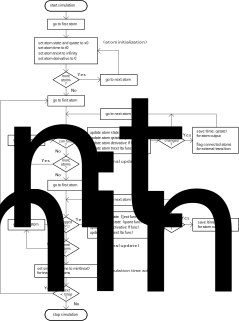
\includegraphics[width=1.0\textwidth]{qdl_flowchart.pdf}
    \caption{Simplified QDL simulation procedure flowchart.}
    \label{fig:qdl_flowchart}
\end{figure}
